\documentclass[11pt]{article}
\usepackage[margin=0.95in,top=0.9in,bottom=0.9in]{geometry}
\usepackage{tikz}
\usetikzlibrary{arrows.meta,positioning,shapes.geometric,calc,fit,backgrounds,decorations.pathreplacing}
\usepackage{booktabs}
\usepackage{amsmath,amssymb}
\usepackage{xcolor}
\usepackage[expansion=false]{microtype}
\usepackage{enumitem}
\usepackage[font=small]{caption}
\usepackage{titlesec}
\usepackage{multicol}
\usepackage[colorlinks=true,linkcolor=blue!55!black,urlcolor=blue!55!black,citecolor=blue!55!black]{hyperref}

\titlespacing*{\section}{0pt}{1.4ex plus .3ex}{0.8ex}
\titlespacing*{\subsection}{0pt}{1.1ex plus .2ex}{0.5ex}
\setlist[itemize]{topsep=2pt,itemsep=1pt,parsep=0pt,leftmargin=1.4em}
\setlist[enumerate]{topsep=2pt,itemsep=1pt,parsep=0pt,leftmargin=1.6em}
\captionsetup{skip=4pt}

\definecolor{cbox}{RGB}{237,242,252}
\definecolor{cline}{RGB}{120,140,175}
\definecolor{mbox}{RGB}{253,240,225}
\definecolor{mline}{RGB}{201,138,71}
\definecolor{gbox}{RGB}{232,245,235}
\definecolor{gline}{RGB}{93,150,110}
\definecolor{rbox}{RGB}{250,235,235}
\definecolor{rline}{RGB}{178,94,94}
\definecolor{note}{RGB}{110,110,120}

\tikzset{
  blk/.style={draw=cline,fill=cbox,rounded corners=2pt,align=center,font=\scriptsize,
              inner sep=3.5pt,minimum height=7.5mm},
  mblk/.style={blk,draw=mline,fill=mbox},
  gblk/.style={blk,draw=gline,fill=gbox},
  rblk/.style={blk,draw=rline,fill=rbox},
  dec/.style={draw=cline,fill=white,diamond,aspect=2.6,align=center,font=\scriptsize,inner sep=1pt},
  ar/.style={-{Stealth[length=4pt]},draw=cline!140,thick},
  lbl/.style={font=\scriptsize\itshape,text=note,inner sep=1.5pt},
}

\newcommand{\M}{\textcolor{blue!45!black}{\scriptsize\textsc{[measured]}}}
\newcommand{\V}{\textcolor{green!35!black}{\scriptsize\textsc{[verified]}}}
\newcommand{\I}{\textcolor{note}{\scriptsize\textsc{[implemented]}}}
\newcommand{\F}{\textcolor{purple!60!black}{\scriptsize\textsc{[inferred]}}}
\newcommand{\Pj}{\textcolor{red!55!black}{\scriptsize\textsc{[projected]}}}
\newcommand{\code}[1]{\texttt{\small #1}}

\begin{document}

\begin{center}
{\LARGE\bfseries Native Word-Level Macro Evaluation\\[2pt] in a GPU RTL Simulator}\\[6pt]
{\large Takneek 2026 $\cdot$ Zenith --- \emph{The Big-GEM Theory}}\\[10pt]
{\normalsize Deliverable E: Scheduling Equations, Memory Architecture,\\
Verification Methodology and Performance Analysis}\\[14pt]
\rule{0.55\textwidth}{0.4pt}\\[6pt]
{\bfseries Done by Pool Shauryas}\\[5pt]
\begin{minipage}{0.8\textwidth}\centering\small
Harshita Bharti \quad$\cdot$\quad Lavanya Prakash \quad$\cdot$\quad Aditi \quad$\cdot$\quad Aahana\\[2pt]
Gauri Singh \quad$\cdot$\quad Soundarya Murugaiyan \quad$\cdot$\quad Dharshini S\\[2pt]
Swadha Singh \quad$\cdot$\quad Ashritha Aryapu
\end{minipage}\\[4pt]
\rule{0.55\textwidth}{0.4pt}
\end{center}

\vspace{2pt}
\noindent\textbf{Abstract.}\;
We extend NVIDIA's GEM boomerang-scheduled GPU logic simulator so that
\code{DSP48E2}, \code{CARRY4} and \code{SRLC32E} primitives survive Yosys synthesis as
word-level cells and are evaluated natively on the GPU ALU using \code{int64\_t}
arithmetic, instead of being shredded into 1-bit AND-inverter logic. The
heterogeneous schedule is defined by two integer labels per graph node,
$\mathrm{avail}$ and $\mathrm{eval}$, whose single point of divergence is the only
synchronisation the design pays for. The implementation is complete for all three
primitives and verified against netlist-level ground truth at every port and every
timestamp. It reduces AIG cell count by $14.8\times$ and the per-cycle instruction
script by $4.53\times$, which carries the script across the L2 capacity and drops DRAM
throughput from $46.91\,\%$ of peak to $0.04\,\%$. End-to-end throughput is
$0.61\times$ the shredded baseline at 16 lanes; the profile attributes the entire
difference to one additional grid synchronisation per simulated cycle, measured two
independent ways, and \S\ref{sec:next} names the single equation term that removes it.

\smallskip
\noindent{\footnotesize\textbf{Evidence tags.}
\M{} instrument output, command in \S\ref{sec:prov}.\;
\V{} compared against an independent reference, with the comparison count stated.\;
\I{} a property of the source, citable to file and line.\;
\F{} a conclusion drawn from named measurements.\;
\Pj{} a prediction, never used to support a performance claim.}

\vspace{-2pt}
{\setcounter{tocdepth}{1}\small\tableofcontents}

\section{Executive Summary}

\textbf{Problem.} GEM attains its throughput by reducing all logic to 1-bit
AND-inverter form, which forces the frontend to shred word-level FPGA primitives.
\M{} One \code{DSP48E2}, four \code{CARRY4} and one \code{SRLC32E} expand from 95 AIG
cells to 9,922 --- $104\times$. GEM re-reads its entire compiled instruction script
from global memory on \emph{every simulated cycle}, so that expansion is paid as
memory bandwidth once per cycle for the life of the run.

\textbf{What we built.} \I{} A macro-preserving path through the whole stack:
Yosys interception (\S\ref{sec:front}), a heterogeneous DAG schedule with two labels
per node (\S\ref{sec:sched}), a warp-padded 64-bit aligned VRAM layout with
CSR-indexed descriptors (\S\ref{sec:vram}), and a macro evaluation phase inside the
boomerang kernel (\S\ref{sec:cuda}). 1,591 lines of new host and device code; GEM's
boomerang reduction tree itself is unmodified.

\textbf{Headline numbers}, \code{macro\_bench} at 16 lanes, RTX 3050 Laptop
(\code{sm\_86}), identical stimulus and identical \code{num\_blocks} on both sides:

\begin{center}\small
\begin{tabular}{lrrl}
\toprule
Quantity & Shredded baseline & Macro-preserving & \\
\midrule
AIG cells                        & 85,444 & \textbf{5,754} & \M{} $14.8\times$ fewer\\
Instruction script, per cycle    & 2,060.0\,KiB & \textbf{454.5\,KiB} & \M{} $4.53\times$ smaller\\
Script vs L2 (1,536\,KiB)        & $1.34\times$ --- spills & $\mathbf{0.30\times}$ --- fits & \M{} residency crossed\\
DRAM throughput (\% of peak)     & 46.91 & \textbf{0.04} & \M{} $1{,}173\times$ less traffic\\
Warps active (\% of peak)        & 33.33 & 33.33 & \M{} occupancy identical\\
Local memory ld/st (sectors)     & 0 & 0 & \M{} nothing spills\\
Grid barriers per simulated cycle& 1 & 2 & \I{} the one added cost\\
\midrule
\textbf{Throughput (cycles/s)}   & \textbf{22,426} & \textbf{13,657} & \M{} $0.61\times$\\
\bottomrule
\end{tabular}
\end{center}

\textbf{Correctness.} \V{} All four rungs of the verification ladder pass on the
16-lane benchmark, 32,800 port$\times$timestamp comparisons each; the
\code{macro\_smoke} regression passes at 49,200. \V{} The three macro models agree
with an independent Python transcription of the problem-statement equations over
14,552 vectors, of which the 1,024 \code{CARRY4} cases are exhaustive.

\textbf{Where the time goes.} \F{} After eliminating memory bandwidth, register
spilling and occupancy against measured quantities, the extra grid barrier is the
only structural difference left between the two configurations. Two independent
timings size it: $37.75\,\mu$s/cycle from the profiler and $31.1\,\mu$s/cycle from
wall clock. \S\ref{sec:next} specifies the change that removes it.

\section{Rubric Coverage}

\begin{center}\footnotesize
\begin{tabular}{@{}p{0.31\textwidth}p{0.42\textwidth}l@{}}
\toprule
Requirement & Implementation & Section\\
\midrule
\multicolumn{3}{@{}l}{\textbf{A --- Host Parser \& Yosys Pre-Processor (15)}}\\
Intercept \code{DSP48E2}/\code{CARRY4}/\code{SRLC32E}
   & \code{synth/gem\_macros.v} (3 blackboxes); \code{macro\_normalize\_xilinx.v} maps real Xilinx ports & \S\ref{sec:front}\\
Prevent techmap / ABC shredding
   & \code{(* blackbox *)} $+$ \code{setattr -set keep 1} in \code{step2\_logic.ys} & \S\ref{sec:front}\\
Yosys 0.68 JSON netlist compatibility
   & \code{write\_json} in both flows; consumed by \code{check\_macros.sh} & \S\ref{sec:front}\\
64-bit aligned, coalesced buffers
   & \code{MacroLayout::build} (\code{macro\_layout.rs:131}), \code{UVec<u64>} & \S\ref{sec:vram}\\
\midrule
\multicolumn{3}{@{}l}{\textbf{B --- CUDA Engine \& Boomerang Modification (35)}}\\
Modified levelized DAG equations
   & \code{macro\_avail\_stage}, \code{staging.rs}, \code{build\_staged\_\dots} & \S\ref{sec:sched}\\
Mixed-width scheduling without stalling warps
   & type-homogeneous \code{MacroBatch}, \code{pe.rs:31} & \S\ref{sec:cuda}\\
Macro$\to$macro ordering ($CO[3]\!\to\!CIN$) without boolean nodes
   & one batch per chain link, \code{ready} vs \code{realized\_inputs}, \code{pe.rs:751} & \S\ref{sec:sched}\\
Native evaluation on the GPU ALU
   & \code{kernel\_v1\_impl.cuh:305--437}; \code{gem\_dsp48e2}, \code{gem\_carry4}, \code{gem\_srlc32e} & \S\ref{sec:cuda}\\
Shared memory \& warp-level primitives
   & \code{shared\_writeouts} hosts macro operands; \code{\_\_shfl\_down\_sync} preserved at 5 sites; \code{\_\_syncthreads()} orders chains & \S\ref{sec:cuda}\\
\midrule
\multicolumn{3}{@{}l}{\textbf{C --- Hardware Macro Implementations (20)}}\\
DSP48E2 subset, PREG-only clocked & \code{gem\_dsp48e2}, \code{csrc/macros.cuh} & \S\ref{sec:macros}\\
CARRY4 exact silicon logic        & \code{gem\_carry4}, \code{macros.cuh:132} & \S\ref{sec:macros}\\
SRLC32E clock-edge semantics      & \code{gem\_srlc32e\_read} / \code{\_edge} & \S\ref{sec:macros}\\
Own behavioural verification, no golden reference supplied
   & \code{csrc/tests/reference\_model.py} $+$ \code{dump\_vectors.cpp} $+$ \code{verify\_macros.sh} & \S\ref{sec:verif}\\
\midrule
\multicolumn{3}{@{}l}{\textbf{D --- Benchmarks \& Performance Analysis (20)}}\\
Throughput vs unmodified GEM, cycles/s & \code{bench/throughput.sh}, \code{bench/sweep.sh} & \S\ref{sec:bench}\\
Memory bandwidth utilisation (Nsight)  & \code{bench/profile.sh}, \code{--replay-mode application} & \S\ref{sec:bench}\\
Warp divergence metrics (Nsight)       & \code{smsp\_\_thread\_inst\_executed} ratio & \S\ref{sec:bench}\\
\midrule
\multicolumn{3}{@{}l}{\textbf{E --- Documentation \& Reports (10)}}\\
Mathematical scheduling equations & Eq.~(1)--(4) with P1--P4 & \S\ref{sec:sched}\\
Architectural block diagrams (Global / Shared / Registers) & Fig.~\ref{fig:mem} & \S\ref{sec:vram}\\
Extensive numerical analysis & \S\ref{sec:bench} & \S\ref{sec:bench}\\
\bottomrule
\end{tabular}
\end{center}

\section{Architecture Overview}

Stock GEM rests on one structural invariant: \emph{every value inside a partition is
produced by the AND-gate cover, and reaches its consumers through the boomerang
hierarchy}. A word-level macro violates it three times over --- it is produced by a
separate evaluation phase, written into a separate buffer, on a separate schedule.
Each consequence is addressed explicitly, and the equations of \S\ref{sec:sched}
exist to restore a well-defined order once the invariant no longer holds.

\begin{figure}[h]\centering
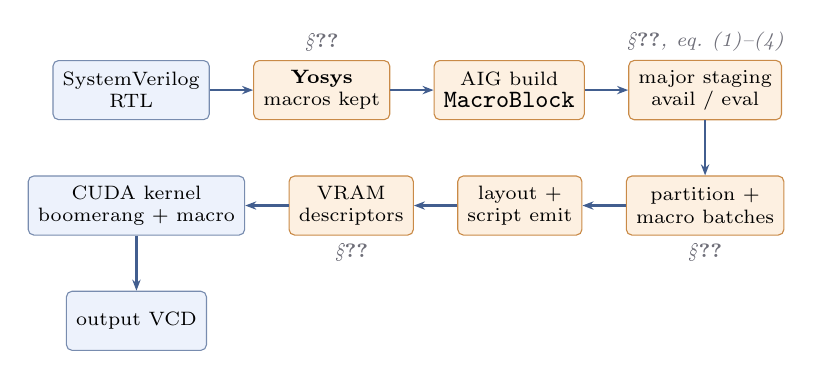
\begin{tikzpicture}[node distance=5.5mm]
\node[blk] (rtl) {SystemVerilog\\RTL};
\node[mblk,right=of rtl] (yos) {\textbf{Yosys}\\macros kept};
\node[mblk,right=of yos] (aig) {AIG build\\\code{MacroBlock}};
\node[mblk,right=of aig] (stage) {major staging\\avail / eval};
\node[mblk,below=7mm of stage] (part) {partition $+$\\macro batches};
\node[mblk,left=of part] (lay) {layout $+$\\script emit};
\node[mblk,left=of lay] (vram) {VRAM\\descriptors};
\node[blk,left=of vram] (ker) {CUDA kernel\\boomerang $+$ macro};
\node[blk,below=7mm of ker] (vcd) {output VCD};
\draw[ar] (rtl)--(yos); \draw[ar] (yos)--(aig); \draw[ar] (aig)--(stage);
\draw[ar] (stage)--(part); \draw[ar] (part)--(lay); \draw[ar] (lay)--(vram);
\draw[ar] (vram)--(ker); \draw[ar] (ker)--(vcd);
\node[lbl,above=0.5mm of yos] {\S\ref{sec:front}};
\node[lbl,above=0.5mm of stage] {\S\ref{sec:sched}, eq.~(1)--(4)};
\node[lbl,below=0.5mm of part] {\S\ref{sec:cuda}};
\node[lbl,below=0.5mm of vram] {\S\ref{sec:vram}};
\end{tikzpicture}
\caption{The compilation pipeline. Shaded stages are new or substantially modified;
the kernel retains GEM's boomerang tree unchanged and gains a macro phase between
write-out settle and commit.}
\label{fig:pipe}
\end{figure}

\section{Host Parser and Yosys Pre-Processor}\label{sec:front}

\I{} \code{synth/gem\_macros.v} declares exactly three blackboxes, and these are the
only macro cell names that ever reach GEM's Rust netlist parser:
\code{\$\_\_GEMDSP\_}, \code{\$\_\_GEMCARRY4\_}, \code{\$\_\_GEMSRL32\_}. The naming
follows GEM's own convention for library macros (\code{\$\_\_RAMGEM\_SYNC\_}), so
\code{src/aigpdk.rs:34} matches on these identifiers and never on Xilinx spellings.

\begin{figure}[h]\centering
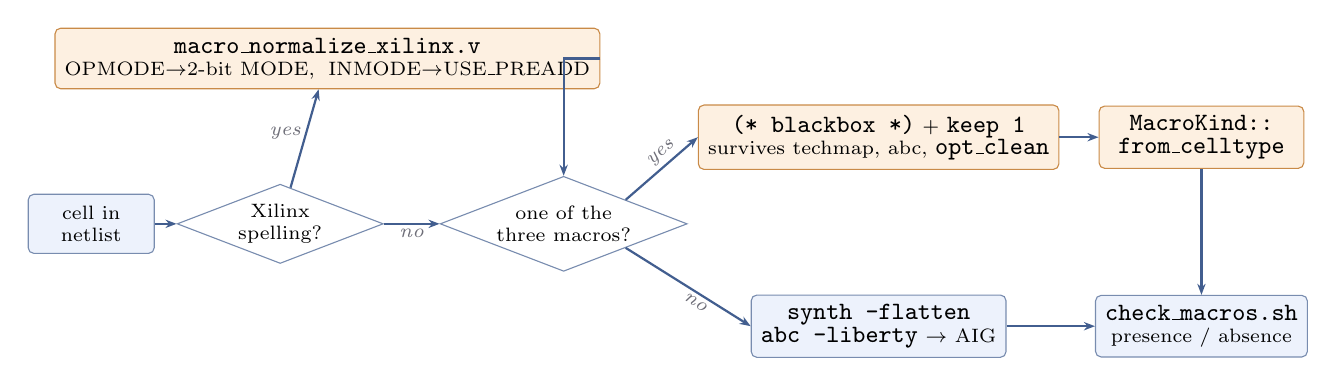
\begin{tikzpicture}[x=1mm,y=1mm]
\node[blk,minimum width=16mm] (cell) at (0,0) {cell in\\netlist};
\node[dec] (isx) at (24,0) {Xilinx\\spelling?};
\node[mblk,minimum width=44mm] (norm) at (30,21)
   {\code{macro\_normalize\_xilinx.v}\\{\scriptsize OPMODE$\to$2-bit MODE,\; INMODE$\to$USE\_PREADD}};
\node[dec] (isg) at (60,0) {one of the\\three macros?};
\node[mblk,minimum width=30mm] (bb) at (100,11) {\code{(* blackbox *)} $+$ \code{keep 1}\\{\scriptsize survives techmap, abc, \code{opt\_clean}}};
\node[blk,minimum width=30mm] (aig) at (100,-13) {\code{synth -flatten}\\\code{abc -liberty} $\to$ AIG};
\node[mblk,minimum width=26mm] (mb) at (141,11) {\code{MacroKind::}\\\code{from\_celltype}};
\node[blk,minimum width=26mm] (chk) at (141,-13) {\code{check\_macros.sh}\\{\scriptsize presence / absence}};
\draw[ar] (cell)--(isx);
\draw[ar] (isx)-- node[lbl,left,pos=0.55]{yes} (norm);
\draw[ar] (norm.east) -| (isg.north);
\draw[ar] (isx)-- node[lbl,below]{no} (isg);
\draw[ar] (isg.north east) -- node[lbl,above,sloped,pos=0.6]{yes} (bb.west);
\draw[ar] (isg.south east) -- node[lbl,below,sloped,pos=0.6]{no} (aig.west);
\draw[ar] (bb)--(mb); \draw[ar] (aig)--(chk); \draw[ar] (mb)--(chk);
\end{tikzpicture}
\caption{Interception. Anything Xilinx-shaped is first normalised to the three
canonical cells, whose port names and widths stay frozen --- so a hidden benchmark
with a different port surface changes one file and nothing else. Everything not
matched takes the ordinary AIG path.}
\label{fig:intercept}
\end{figure}

\textbf{Why the macros survive.} \I{} Two mechanisms, both necessary: a blackbox has
no body, so \code{synth -flatten} cannot inline it and \code{abc -liberty} treats the
instance as a cone boundary exactly like a DFF; and \code{setattr -set keep 1}
prevents \code{opt\_clean -purge} from sweeping it as dead logic.

\textbf{A falsifiable baseline.} \V{} \code{synth/run\_synth.sh} builds \emph{both}
flows from identical RTL, and \code{check\_macros.sh} asserts the opposite condition
in each: macros \textbf{present} in the native \code{gatelevel.json}, \textbf{absent}
in the shredded one, with a non-zero exit if a macro ever survives into the baseline.
Without this the entire throughput comparison in \S\ref{sec:bench} could be void
while still producing plausible numbers.

\textbf{Mapping macro nodes into GEM.} \I{} \code{MacroKind::from\_celltype}
(\code{src/aig.rs:393}) recognises the three cells during the netlist DFS, and
establishes two properties relied on everywhere downstream. \emph{Topological order
by construction:} the DFS resolves a macro's combinational fan-in before allocating
its output aigpin, so a macro output is always above its inputs --- GEM's levelization
assumes this. \emph{Ports addressed by canonical slot, not netlist iteration order:}
\code{MacroBlock.in\_iv} is indexed by \code{MacroKind::input\_slot}, so \code{CARRY4}
is always $S[0..3], DI[0..3], CIN, CYINIT$ regardless of the order Yosys emitted pins.
\V{} Unit test \code{canonical\_order\_tests} asserts the Rust tables and
\code{gem\_macros.v} agree: if a width moves in one place it must move in the other.

\section{Modified DAG Levelization Equations}\label{sec:sched}

Let $G=(V,E)$ be the AND-inverter graph after macro-preserving synthesis; each
$v \in V$ is an \emph{aigpin}. Write $\mathrm{fanin}(v)$ for the AND-gate fan-in;
$\mathcal{M}$ for the macro instances; $\mathrm{combin}(m)$ for the
\emph{combinational} input pins of macro $m$ (\code{CARRY4}: $S,DI,CIN,CYINIT$;
\code{SRLC32E}: $A[4{:}0]$; \code{DSP48E2}: $\emptyset$); $\mathcal{O}_c \subset V$
for aigpins driven by a combinational macro output ($CO,O,Q,Q_{31}$); and
$\mathcal{O}_s \subset V$ for aigpins driven by a clocked macro output ($P$).

Two integer labels per node. They coincide everywhere except on $\mathcal{O}_c$, and
that single point of divergence is the entire content of the heterogeneous schedule:
$\mathrm{avail}(v)$ is the major stage in which $v$ may be \emph{read} by boolean
logic, and $\mathrm{eval}(v)$ the major stage in which the producer of $v$ is
\emph{executed}.

\vspace{-2pt}
\begin{align}
\mathrm{avail}(v) &= 0, && v \text{ a primary input, DFF } Q,\ \text{SRAM read data, or } v \in \mathcal{O}_s\\
\mathrm{avail}(v) &= \max_{u \in \mathrm{fanin}(v)} \mathrm{avail}(u), && v \text{ an AND gate}\\
\mathrm{eval}(m) &= \max_{p \in \mathrm{combin}(m)}
   \begin{cases} \mathrm{eval}(p) & p \in \mathcal{O}_c\\ \mathrm{avail}(p) & \text{otherwise}\end{cases}, && m \in \mathcal{M}\\
\mathrm{avail}(v) &= \mathrm{eval}(m) + 1, && v \in \mathcal{O}_c \text{ driven by } m
\end{align}

\begin{figure}[h]\centering
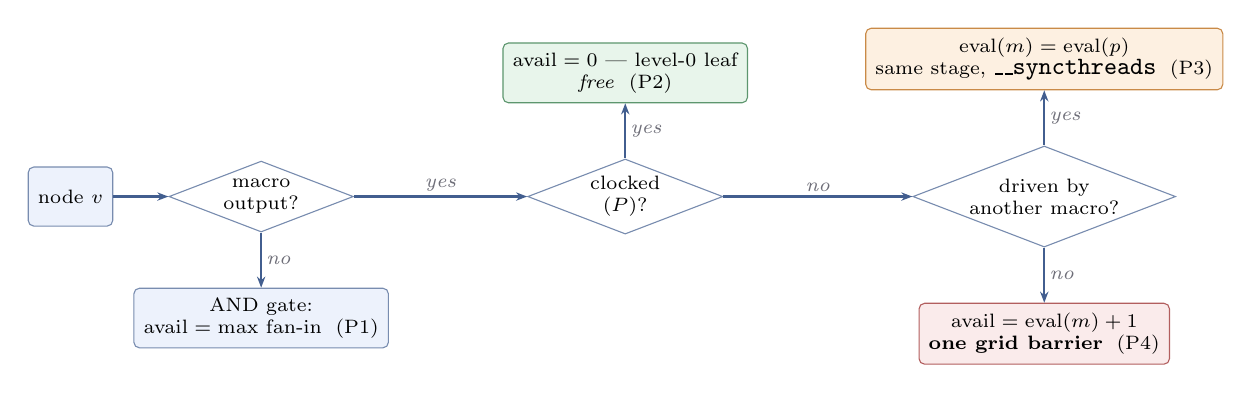
\begin{tikzpicture}[node distance=5mm]
\node[blk] (n) {node $v$};
\node[dec,right=7mm of n] (d1) {macro\\output?};
\node[blk,below=7mm of d1] (and) {AND gate:\\$\mathrm{avail}=\max$ fan-in \;(P1)};
\node[dec,right=22mm of d1] (d2) {clocked\\($P$)?};
\node[gblk,above=7mm of d2] (clk) {$\mathrm{avail}=0$ --- level-0 leaf\\\emph{free} \;(P2)};
\node[dec,right=24mm of d2] (d3) {driven by\\another macro?};
\node[mblk,above=7mm of d3] (chain) {$\mathrm{eval}(m)=\mathrm{eval}(p)$\\same stage, \code{\_\_syncthreads} \;(P3)};
\node[rblk,below=7mm of d3] (cross) {$\mathrm{avail}=\mathrm{eval}(m)+1$\\\textbf{one grid barrier} \;(P4)};
\draw[ar] (n)--(d1);
\draw[ar] (d1)-- node[lbl,right]{no} (and);
\draw[ar] (d1)-- node[lbl,above]{yes} (d2);
\draw[ar] (d2)-- node[lbl,right]{yes} (clk);
\draw[ar] (d2)-- node[lbl,above]{no} (d3);
\draw[ar] (d3)-- node[lbl,right]{yes} (chain);
\draw[ar] (d3)-- node[lbl,right]{no} (cross);
\end{tikzpicture}
\caption{How a node acquires its labels. Three of the four paths are free; only the
last --- a combinational macro result crossing into the AND-gate domain --- costs a
major stage, and it is charged exactly once.}
\label{fig:labels}
\end{figure}

\textbf{(P1) Boolean depth is free.} Eq.~(2) takes a maximum, never an increment: an
arbitrarily deep cone of AND gates evaluates inside one major stage, exactly as in
stock GEM. The boomerang hierarchy is untouched.

\textbf{(P2) Clocked macro outputs cost nothing.} By eq.~(1), $\mathcal{O}_s$ is a
level-0 leaf. A DSP's $P$ is read from global state like a DFF's $Q$: what a reader
observes this cycle is last cycle's commit, which is the correct register semantics
and requires no boundary.

\textbf{(P3) Macro-to-macro chaining costs nothing.} The case split in eq.~(3) takes
\emph{eval}, not \emph{avail}, of an operand that is itself a combinational macro
output. Hence a \code{CARRY4} chain of any length --- $CO[3]\!\to\!CIN$, the
dependency the problem statement names explicitly --- resolves inside a single major
stage, ordered by one batch per chain link separated by \code{\_\_syncthreads()}.
Without this case split a 64-bit carry-chain adder would demand 16 major stages.

\textbf{(P4) Only macro-to-boolean pays.} The $+1$ in eq.~(4) is charged once, and
only where a combinational macro result must cross into the AND-gate domain --- the
minimum price consistent with the buffer separation described above.

\textbf{Stage construction.} With $D = \max_v \mathrm{eval}(v)$ over endpoints, major
stage $j \in [0,D]$ is defined by
\begin{align}
\mathrm{endpoints}(j) &= \{e : \textstyle\max_{p \in \mathrm{inputs}(e)} \mathrm{avail}(p) = j\}\\
\mathrm{macros}(j) &= \{m \in \mathcal{M} : \mathrm{eval}(m) = j\}\\
\mathrm{forward}(j) &= \{v : \mathrm{eval}(v) \le j \;\wedge\; \exists\, c \in \mathrm{consumers}(v),\ \mathrm{eval}(c) > j\}
\end{align}
The second clause of $\mathrm{forward}(j)$ is the subtle one: a node with
$\mathrm{eval}(v)=j$ but $\mathrm{avail}(v)=j{+}1$ --- a combinational macro output
produced by stage $j$'s macro phase --- must be forwarded even though it is not
readable in the stage that produces it.

\textbf{Regression guarantee.} \I{} If $\mathcal{O}_c = \emptyset$ then $D=0$ by
construction and a macro-free netlist is scheduled bit-identically to stock GEM.
This is what makes the baseline comparison in \S\ref{sec:bench} meaningful rather
than circular, and it is asserted by unit test
\code{nothing\_but\_a\_combinational\_macro\_can\_raise\_a\_stage}.

\textbf{Measured instantiation.} \M{} On \code{bench/macro\_bench.sv} at
$\mathrm{LANES}=16$ --- 16 \code{DSP48E2}, 64 \code{CARRY4} in 16 four-block chains,
16 \code{SRLC32E}, 96 macros in all --- the equations yield $D=1$, and the 64 chained
\code{CARRY4}s occupy \emph{four batches within one major stage} rather than four
stages:

\begin{center}\small
\begin{tabular}{clrr}
\toprule
Major stage & Contents & Partitions & Macro batches\\
\midrule
0 & 16 \code{DSP48E2} (endpoint), 64 \code{CARRY4}, 16 \code{SRLC32E} & 2 & 5\\
1 & boolean cones consuming macro results & 1 & 0\\
\bottomrule
\end{tabular}
\end{center}

This is (P3) doing the work it exists for. Had chaining been charged a major stage
per link, this design would have needed five stages instead of two, and
\S\ref{sec:bench} shows each additional major stage costs $\approx 31\,\mu$s per
simulated cycle --- so (P3) is worth roughly $93\,\mu$s/cycle on a design this shape.

\begin{figure}[h]\centering
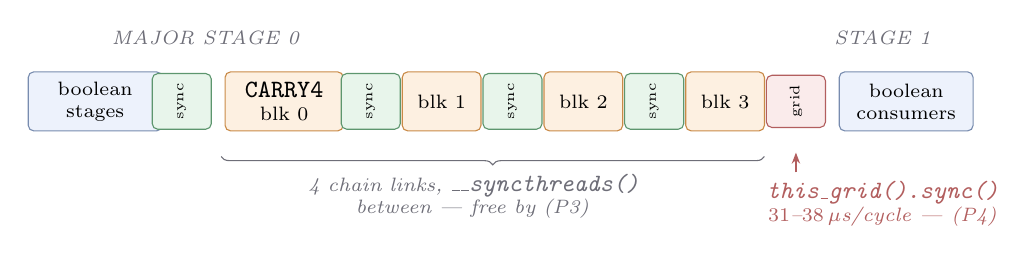
\begin{tikzpicture}[x=1mm,y=1mm]
\node[blk,minimum width=17mm] (b0) at (0,0) {boolean\\stages};
\node[gblk,minimum width=4mm,font=\tiny,rotate=90] (s1) at (11,0) {sync};
\node[mblk,minimum width=15mm] (c0) at (24,0) {\code{CARRY4}\\blk 0};
\node[gblk,minimum width=4mm,font=\tiny,rotate=90] (s2) at (35,0) {sync};
\node[mblk,minimum width=10mm] (c1) at (44,0) {blk 1};
\node[gblk,minimum width=4mm,font=\tiny,rotate=90] (s3) at (53,0) {sync};
\node[mblk,minimum width=10mm] (c2) at (62,0) {blk 2};
\node[gblk,minimum width=4mm,font=\tiny,rotate=90] (s4) at (71,0) {sync};
\node[mblk,minimum width=10mm] (c3) at (80,0) {blk 3};
\node[rblk,minimum width=5mm,font=\tiny,rotate=90] (g) at (89,0) {grid};
\node[blk,minimum width=17mm] (b1) at (103,0) {boolean\\consumers};
\node[lbl] at (14,8) {MAJOR STAGE 0};
\node[lbl] at (100,8) {STAGE 1};
\draw[decorate,decoration={brace,amplitude=3pt,mirror},draw=note] (16,-7) -- (85,-7);
\node[lbl,text width=62mm,align=center] at (48,-12)
  {4 chain links, \code{\_\_syncthreads()} between --- free by (P3)};
\draw[ar,draw=rline] (89,-9) -- (89,-6.5);
\node[lbl,text=rline,align=center] at (100,-13) {\code{this\_grid().sync()}\\$31$--$38\,\mu$s/cycle --- (P4)};
\end{tikzpicture}
\caption{One simulated cycle. Chaining is ordered by block-level fences, which cost
nothing measurable; only the macro$\to$boolean edge forces a grid-wide barrier.}
\label{fig:cycle}
\end{figure}

\section{VRAM Layout Architecture}\label{sec:vram}

The organising principle is \emph{lifetime}, not macro identity. A value that must
survive to the next simulated cycle goes to global memory; a value consumed within
the cycle that produced it never leaves shared memory; the arithmetic itself happens
in registers, where nothing is addressable at all.

\begin{figure}[h]\centering
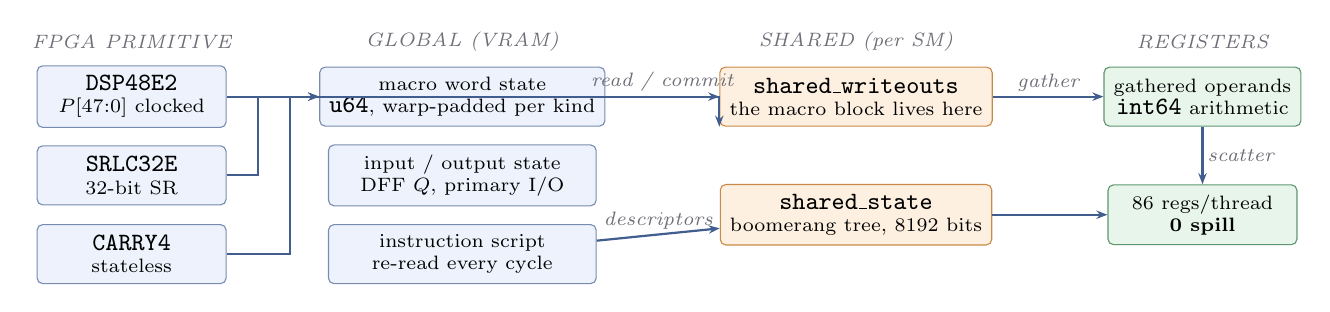
\begin{tikzpicture}[x=1mm,y=1mm]
\node[lbl] at (0,13) {FPGA PRIMITIVE};
\node[blk,minimum width=24mm] (dsp) at (0,6) {\code{DSP48E2}\\{\scriptsize$P[47{:}0]$ clocked}};
\node[blk,minimum width=24mm] (srl) at (0,-4) {\code{SRLC32E}\\{\scriptsize 32-bit SR}};
\node[blk,minimum width=24mm] (c4)  at (0,-14) {\code{CARRY4}\\{\scriptsize stateless}};
\node[lbl] at (42,13) {GLOBAL (VRAM)};
\node[blk,minimum width=34mm] (gw)  at (42,6) {macro word state\\{\scriptsize\code{u64}, warp-padded per kind}};
\node[blk,minimum width=34mm] (gio) at (42,-4) {input / output state\\{\scriptsize DFF $Q$, primary I/O}};
\node[blk,minimum width=34mm] (gs)  at (42,-14) {instruction script\\{\scriptsize re-read every cycle}};
\node[lbl] at (92,13) {SHARED (per SM)};
\node[mblk,minimum width=32mm] (sw) at (92,6) {\code{shared\_writeouts}\\{\scriptsize the macro block lives here}};
\node[mblk,minimum width=32mm] (ss) at (92,-9) {\code{shared\_state}\\{\scriptsize boomerang tree, 8192 bits}};
\node[lbl] at (136,13) {REGISTERS};
\node[gblk,minimum width=24mm] (r1) at (136,6) {gathered operands\\{\scriptsize \code{int64} arithmetic}};
\node[gblk,minimum width=24mm] (r2) at (136,-9) {86 regs/thread\\{\scriptsize \textbf{0 spill}}};
\draw[ar] (dsp)--(gw);
\draw[ar] (srl.east) -- ++(4mm,0) |- (gw.west);
\draw[ar] (c4.east) -- ++(8mm,0) -- ++(0,20mm) -| (sw.south west);
\draw[ar] (gw)-- node[lbl,above]{read / commit} (sw);
\draw[ar] (sw)-- node[lbl,above]{gather} (r1);
\draw[ar] (gs)-- node[lbl,above]{descriptors} (ss);
\draw[ar] (ss)--(r2);
\draw[ar] (r1)-- node[lbl,right]{scatter} (r2);
\end{tikzpicture}
\caption{Where each primitive's state and operands physically live. Split by
lifetime: state that survives the cycle is global, values consumed within it stay
shared, arithmetic happens in registers. A \code{CARRY4} is stateless and therefore
never touches global memory at all.}
\label{fig:mem}
\end{figure}

\textbf{Two disjoint regions.} \I{} \emph{Bit-addressed outputs} live in the
partition's write-out block, interleaved with ordinary boolean write-outs so the
existing commit path carries them to global state with no separate store.
\emph{Word-addressed internal state} --- a DSP's $PREG$, an SRLC32E's 32-bit shift
register --- lives in a dedicated \code{UVec<u64>} region, \code{macro\_word\_state}.

\begin{figure}[h]\centering
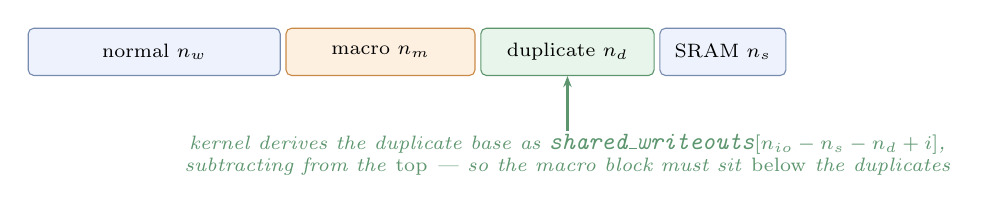
\begin{tikzpicture}[x=1mm,y=1mm]
\node[blk,minimum width=32mm,minimum height=6mm] (n) at (0,0) {normal $n_w$};
\node[mblk,minimum width=24mm,minimum height=6mm,right=0.6mm of n] (m) {macro $n_m$};
\node[gblk,minimum width=22mm,minimum height=6mm,right=0.6mm of m] (d) {duplicate $n_d$};
\node[blk,minimum width=16mm,minimum height=6mm,right=0.6mm of d] (s) {SRAM $n_s$};
\draw[ar,draw=gline] ($(d.south)+(0,-7mm)$) -- (d.south);
\node[lbl,text=gline,align=center] at ($(d.south)+(0,-10mm)$)
  {kernel derives the duplicate base as \code{shared\_writeouts}$[n_{io}-n_s-n_d+i]$,\\
   subtracting from the \emph{top} --- so the macro block must sit \emph{below} the duplicates};
\end{tikzpicture}
\caption{Write-out region ordering. SRAM stays last so its pre-existing offset
arithmetic is untouched; the macro block sits below the duplicates because the kernel
locates duplicates by subtracting from the top of the region. This is a correctness
requirement, not a layout preference.}
\label{fig:order}
\end{figure}

\textbf{Slot allocation.} Macro instance $i$ receives
$n_{\mathrm{slots}}(i) = \lceil |\mathrm{outputs}(i)| / 32 \rceil$ contiguous
\code{u32} slots, so bit $b$ lands at global state bit
$32\cdot \mathrm{macro\_start}_i + b$. Two consequences fall out of the allocation
rather than from a convention: every macro's output field is contiguous and 32-bit
aligned, and because each macro owns whole words, no two macros can contend for the
same \code{u32} --- so the device-side result scatter is a plain read-modify-write
requiring \textbf{no atomics}.

\textbf{Alignment.} \I{} The word-state region is a \code{UVec<u64>}: the element type
supplies 8-byte alignment and \code{cudaMalloc} a 256-byte aligned base, so the
problem statement's 64-bit alignment requirement holds \emph{structurally} rather
than by runtime assertion. Instances are grouped by kind and each kind begins on a
warp boundary, so a type-homogeneous batch reads a contiguous, segment-aligned span
--- the condition for coalesced access.

\textbf{Script-side indirection.} A batch record references macros by index into the
layout's slot table rather than inlining descriptors (a DSP descriptor alone is 176
words; inlining would dwarf the script it lives in): \code{[stage index | kind code |
count | count $\times$ slot index]}. \M{} Measured effect on \code{macro\_smoke}: the
macro-preserving script is \textbf{69,652} words against the baseline's
\textbf{94,720} --- a $26\,\%$ reduction, the direct instruction-memory dividend of
not shredding. \M{} Layout totals: 7 instances, $64\times$\code{u64} $=512$ bytes of
word state, 458 descriptor words, 9 macro write-out slots.

\section{CUDA Execution Engine}\label{sec:cuda}

\I{} \code{csrc/kernel\_v1\_impl.cuh:305--437}. The macro phase runs \emph{after} the
boolean write-outs have settled in \code{shared\_writeouts} and \emph{before} they are
committed to \code{output\_state}. A macro therefore reads its operands from what
this partition has just produced and drops its results into the same write-out block;
the existing commit path carries them out, the clock-enable machinery applies
unchanged, and the boomerang reduction tree is not modified.

\begin{figure}[h]\centering
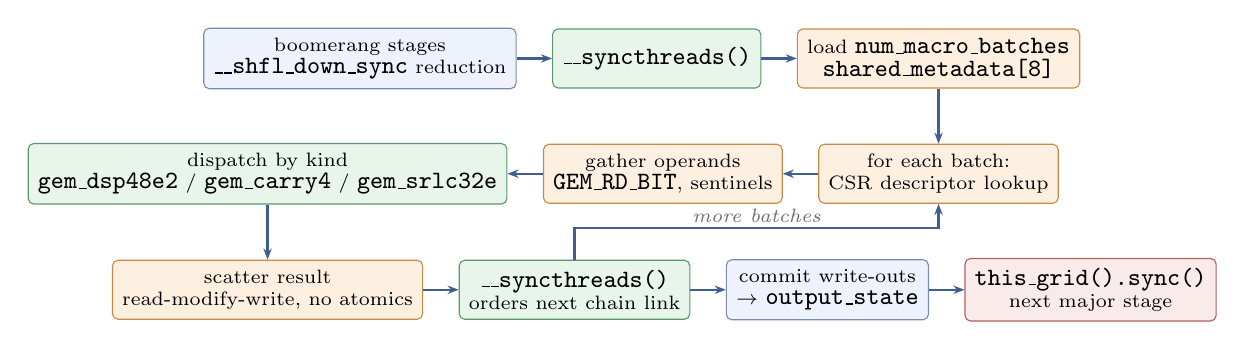
\begin{tikzpicture}[node distance=4.5mm]
\node[blk] (a) {boomerang stages\\{\scriptsize \code{\_\_shfl\_down\_sync} reduction}};
\node[gblk,right=of a] (b) {\code{\_\_syncthreads()}};
\node[mblk,right=of b] (c) {load \code{num\_macro\_batches}\\{\scriptsize \code{shared\_metadata[8]}}};
\node[mblk,below=7mm of c] (d) {for each batch:\\{\scriptsize CSR descriptor lookup}};
\node[mblk,left=of d] (e) {gather operands\\{\scriptsize \code{GEM\_RD\_BIT}, sentinels}};
\node[gblk,left=of e] (f) {dispatch by kind\\{\scriptsize \code{gem\_dsp48e2} / \code{gem\_carry4} / \code{gem\_srlc32e}}};
\node[mblk,below=7mm of f] (g) {scatter result\\{\scriptsize read-modify-write, no atomics}};
\node[gblk,right=of g] (h) {\code{\_\_syncthreads()}\\{\scriptsize orders next chain link}};
\node[blk,right=of h] (i) {commit write-outs\\{\scriptsize $\to$ \code{output\_state}}};
\node[rblk,right=of i] (j) {\code{this\_grid().sync()}\\{\scriptsize next major stage}};
\draw[ar] (a)--(b); \draw[ar] (b)--(c); \draw[ar] (c)--(d); \draw[ar] (d)--(e);
\draw[ar] (e)--(f); \draw[ar] (f)--(g); \draw[ar] (g)--(h);
\draw[ar] (h.north) -- ++(0,4mm) -| node[lbl,above,pos=0.25]{more batches} (d.south);
\draw[ar] (h)--(i); \draw[ar] (i)--(j);
\end{tikzpicture}
\caption{The macro phase inside one partition, per simulated cycle. Batches are
type-homogeneous, so every active lane in a batch takes the same \code{switch} arm and
the warp does not diverge across kinds.}
\label{fig:kernel}
\end{figure}

\begin{center}\footnotesize
\begin{tabular}{@{}p{0.17\textwidth}p{0.24\textwidth}p{0.28\textwidth}p{0.24\textwidth}@{}}
\toprule
Mechanism & Where & Purpose & Measured consequence\\
\midrule
\code{\_\_shfl\_down\_sync} & 5 sites: boomerang reduction, SRAM gather & warp-scope reduction of the 13-level tree & \M{} preserved in both configurations\\
\code{\_\_syncthreads()} & between macro batches, around the phase & order a chained macro against its producer & \M{} below profiler noise\\
Shared memory & \code{shared\_writeouts} & macro operands and results, no global round-trip & \M{} 3,328 B/block; not the occupancy limiter\\
Registers & gathered operands, \code{int64} arithmetic & native word-level ALU work & \M{} 86 regs, \textbf{0 spill}\\
\code{this\_grid().sync()} & between major stages & make a macro result visible to boolean logic & \M{} $37.75\,\mu$s/cycle --- dominant cost\\
\bottomrule
\end{tabular}
\end{center}

\textbf{Why block scope, not warp scope, for the macro fence.} \I{} The macro phase
deliberately does not use a warp shuffle for its own ordering, and this is a scope
argument rather than an omission. Within a batch, macros are mutually independent by
construction --- \code{pe.rs} computes \code{ready} against \code{realized\_inputs}
\emph{before} updating it, so a chained consumer cannot share a batch with its
producer. The ordering requirement is therefore \emph{between} batches, and \M{} a
batch can exceed 32 macros (64 \code{CARRY4} in one partition at 16 lanes), so the
fence must be block-scope; a warp shuffle cannot express it. GEM's own warp-level
primitives are preserved unchanged at all five sites where they already existed.

\textbf{Occupancy and registers.} \M{} Measured with \code{cuobjdump -res-usage} on
the shipped \code{sm\_86} binary: 86 and 105 registers/thread across the two compiled
variants, \textbf{0 bytes} stack and local memory in both, 3,328 B shared, 2 blocks/SM
either way --- a cooperative grid ceiling of $2\times 20 = 40$ blocks, which is exactly
the \code{num\_blocks} used. \code{-maxrregcount} \emph{caps} allocation rather than
permitting growth, so additional pressure would spill silently instead of failing to
launch; the local-memory counter reading zero is what proves it did not.

\section{Hardware Macro Implementations}\label{sec:macros}

\I{} All three live in \code{csrc/macros.cuh}, compiled with
\code{\_\_host\_\_ \_\_device\_\_ \_\_forceinline\_\_}, so one source serves the CPU
executor and the GPU kernel and the two models cannot drift apart.

\begin{figure}[h]\centering
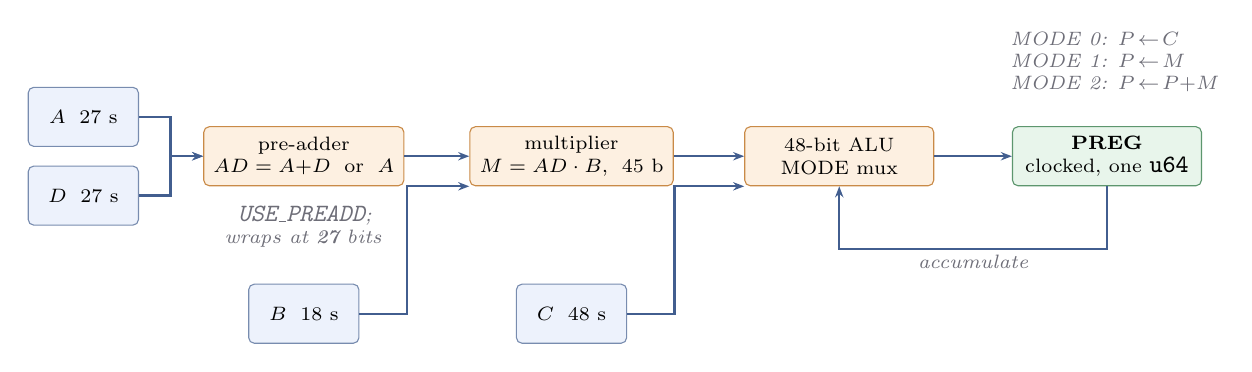
\begin{tikzpicture}[x=1mm,y=1mm]
\node[blk,minimum width=14mm] (a) at (0,4)  {$A$ \;27 s};
\node[blk,minimum width=14mm] (d) at (0,-6) {$D$ \;27 s};
\node[mblk,minimum width=24mm] (pre) at (28,-1) {pre-adder\\{\scriptsize $AD=A{+}D$ \;or\; $A$}};
\node[blk,minimum width=14mm] (b) at (28,-21) {$B$ \;18 s};
\node[mblk,minimum width=24mm] (mul) at (62,-1) {multiplier\\{\scriptsize $M=AD\cdot B$, \;45 b}};
\node[blk,minimum width=14mm] (c) at (62,-21) {$C$ \;48 s};
\node[mblk,minimum width=24mm] (alu) at (96,-1) {48-bit ALU\\{\scriptsize MODE mux}};
\node[gblk,minimum width=24mm] (p) at (130,-1) {\textbf{PREG}\\{\scriptsize clocked, one \code{u64}}};
\node[lbl,align=left] at (131,11) {MODE 0: $P\!\leftarrow\!C$\\MODE 1: $P\!\leftarrow\!M$\\MODE 2: $P\!\leftarrow\!P{+}M$};
\node[lbl,align=center,text width=26mm] at (28,-10) {\code{USE\_PREADD};\\wraps at \textbf{27} bits};
\draw[ar] (a.east) -- ++(4mm,0) |- (pre.west);
\draw[ar] (d.east) -- ++(4mm,0) |- (pre.west);
\draw[ar] (pre)--(mul);
\draw[ar] (b.east) -- ++(6mm,0) |- (mul.south west);
\draw[ar] (mul)--(alu);
\draw[ar] (c.east) -- ++(6mm,0) |- (alu.south west);
\draw[ar] (alu)--(p);
\draw[ar] (p.south) -- ++(0,-8mm) -| node[lbl,below,pos=0.25]{accumulate} (alu.south);
\end{tikzpicture}
\caption{\code{DSP48E2} subset. All input and internal registers are combinational per
the problem statement; only $P$ is clocked, one \code{u64} of state per instance, and
$P$ commits solely when the traced clock enable is high.}
\label{fig:dsp}
\end{figure}

\textbf{DSP48E2.} \I{} $AD = (A+D) \bmod 2^{27}$ signed, $M = AD \times B$ (45 bits),
then $P_{\text{next}} \in \{C, M, P_{\text{cur}}+M\}$ by \code{MODE}, truncated to 48
bits. The pre-adder width is the subtle case and has its own directed vectors:
$A=D=2^{26}-1$ sums to $2^{27}-2$, which is $-2$ once the 27-bit pre-adder truncates.
\V{} 1,648 vectors --- 12 directed (signed extremes, both pre-adder paths, all three
modes, the wrap case) plus 400 random, each accumulated over 4 cycles so PREG feedback
and 48-bit wrap are exercised.

\begin{figure}[h]\centering
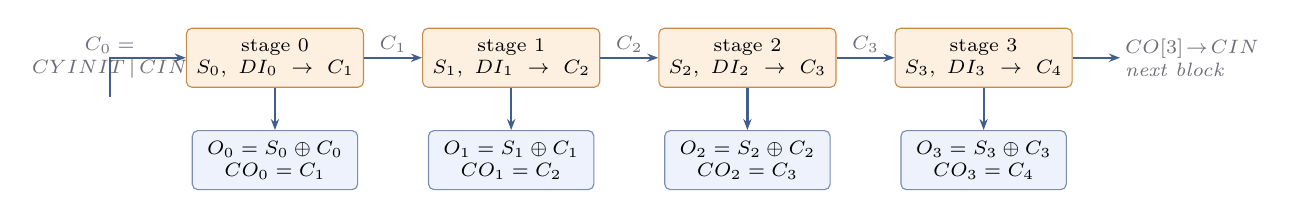
\begin{tikzpicture}[x=1mm,y=1mm]
\node[lbl,align=center] at (-21,4) {$C_0 =$\\$CYINIT \,|\, CIN$};
\foreach \i in {0,1,2,3} {
  \pgfmathsetmacro\x{\i*30}
  \pgfmathtruncatemacro\j{\i+1}
  \node[mblk,minimum width=21mm] (m\i) at (\x,4) {stage \i\\{\scriptsize $S_\i,\ DI_\i \ \to\ C_{\j}$}};
  \node[blk,minimum width=21mm] (o\i) at (\x,-9) {{\scriptsize $O_\i=S_\i\oplus C_\i$}\\{\scriptsize $CO_\i=C_{\j}$}};
  \draw[ar] (m\i)--(o\i);
}
\draw[ar] (-21,-1)|-(m0.west);
\draw[ar] (m0)-- node[lbl,above]{$C_1$} (m1);
\draw[ar] (m1)-- node[lbl,above]{$C_2$} (m2);
\draw[ar] (m2)-- node[lbl,above]{$C_3$} (m3);
\draw[ar] (m3.east) -- ++(6mm,0) node[lbl,right,align=left]{$CO[3]\!\to\! CIN$\\next block};
\end{tikzpicture}
\caption{\code{CARRY4}, transcribed directly from the problem statement:
$C_{i+1} = (S_i \wedge C_i) \vee (\neg S_i \wedge DI_i)$, with
$O_i = S_i \oplus C_i$ and $CO_i = C_{i+1}$. Stateless; the eight output bits are
packed as $CO \,|\, (O \ll 4)$ into one \code{u32} write-out slot.
\V{} Verified \textbf{exhaustively} over all 1,024 input combinations.}
\label{fig:c4}
\end{figure}

\textbf{SRLC32E.} \I{} Inputs $D$, $CE$, $A[4{:}0]$; state is a 32-bit shift register in
one \code{u64} slot. Combinational read $Q = SR[A]$, $Q_{31} = SR[31]$; on the edge, if
$CE$ then $SR \leftarrow (SR \ll 1) \,|\, D$. The ordering is GEM's read-old /
commit-new discipline, exactly as the DFF path does it:
\code{gem\_srlc32e\_read} is called \emph{before} \code{gem\_srlc32e\_edge} within a
cycle, so a reader sees the pre-shift state. \V{} 11,520 read vectors (60 random start
states $\times$ 6 shift steps $\times$ all 32 addresses --- every address exercised at
every step) plus 360 edge vectors.

\begin{center}\small
\begin{tabular}{lrll}
\toprule
Primitive & Vectors & Coverage & Result\\
\midrule
\code{CARRY4}   & 1,024  & \textbf{exhaustive} & \V{} 0 disagreements\\
\code{DSP48E2}  & 1,648  & directed $+$ random, 4-cycle accumulate & \V{} 0 disagreements\\
\code{SRLC32E}  & 11,880 & every address $\times$ every step & \V{} 0 disagreements\\
\midrule
\textbf{Total}  & \textbf{14,552} & & \\
\bottomrule
\end{tabular}
\end{center}

\I{} The comparison is cross-language and cross-implementation:
\code{csrc/tests/dump\_vectors.cpp} emits results from the CUDA models;
\code{csrc/tests/reference\_model.py} computes the same set independently from the
problem-statement equations; \code{verify\_macros.sh} diffs them. The two share only
the LCG that generates the random inputs.

\section{Verification Methodology}\label{sec:verif}

No golden reference was supplied, so correctness rests on oracles that share no code
with the thing they validate. The ladder below isolates one layer per rung, so a
disagreement names the layer that caused it rather than merely reporting a wrong
waveform.

\begin{figure}[h]\centering
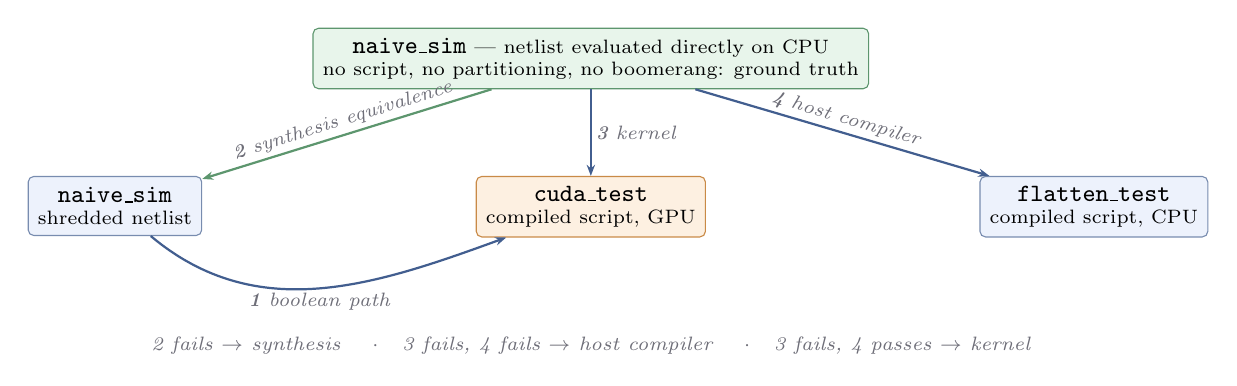
\begin{tikzpicture}[node distance=8mm]
\node[gblk,minimum width=42mm] (gt) {\code{naive\_sim} --- netlist evaluated directly on CPU\\{\scriptsize no script, no partitioning, no boomerang: ground truth}};
\node[blk,below left=11mm and 14mm of gt] (ns) {\code{naive\_sim}\\shredded netlist};
\node[mblk,below=11mm of gt] (gpu) {\code{cuda\_test}\\compiled script, GPU};
\node[blk,below right=11mm and 14mm of gt] (ft) {\code{flatten\_test}\\compiled script, CPU};
\draw[ar,draw=gline] (gt) -- node[lbl,above,sloped]{\textbf{2} synthesis equivalence} (ns);
\draw[ar] (gt) -- node[lbl,right]{\textbf{3} kernel} (gpu);
\draw[ar] (gt) -- node[lbl,above,sloped]{\textbf{4} host compiler} (ft);
\draw[ar] (ns) to[out=-40,in=200] node[lbl,below]{\textbf{1} boolean path} (gpu);
\node[lbl,below=12mm of gpu,align=center]
  {2 fails $\to$ synthesis \quad$\cdot$\quad 3 fails, 4 fails $\to$ host compiler
   \quad$\cdot$\quad 3 fails, 4 passes $\to$ kernel};
\end{tikzpicture}
\caption{Rung 2 is the one no GPU-only comparison can supply: it establishes that both
netlists are the same design before a GPU is involved. Rung 4 bisects rung 3, which
is what made the remaining defects findable in seconds rather than through GPU
round-trips.}
\label{fig:ladder}
\end{figure}

\begin{center}\small
\begin{tabular}{@{}llrl@{}}
\toprule
Rung & What it isolates & Comparisons & Result\\
\midrule
Macro models & PS equations, C++ vs Python & 14,552 vectors & \V{} \textbf{Pass}\\
\multicolumn{4}{@{}l}{\emph{\code{macro\_bench}, $\mathrm{LANES}=16$ --- 82 ports $\times$ 400 cycles}}\\
1. Shredded GPU vs \code{naive\_sim}   & the ordinary boolean path      & 32,800 & \V{} \textbf{Pass}\\
2. Design equivalence (CPU only)       & macro-preserving synthesis     & 32,800 & \V{} \textbf{Pass}\\
3. Macro GPU vs \code{naive\_sim}      & the CUDA kernel                & 32,800 & \V{} \textbf{Pass}\\
4. Compiled script vs \code{naive\_sim}& \code{pe.rs} / \code{flatten.rs} & 32,800 & \V{} \textbf{Pass}\\
\multicolumn{4}{@{}l}{\emph{\code{macro\_smoke} regression --- 123 ports $\times$ 400 cycles}}\\
2. Design equivalence (CPU only)       & macro-preserving synthesis     & 49,200 & \V{} \textbf{Pass}\\
4. Compiled script vs \code{naive\_sim}& \code{pe.rs} / \code{flatten.rs} & 49,200 & \V{} \textbf{Pass}\\
\bottomrule
\end{tabular}
\end{center}

On \code{macro\_bench} the macro-preserving path evaluates 16 \code{DSP48E2}, 64
\code{CARRY4} --- including 16 four-deep $CO[3]\!\to\!CIN$ chains --- and 16
\code{SRLC32E} natively on the GPU ALU, and reproduces netlist-level ground truth at
every port and every timestamp. One dependency in that design exists purely as a
regression test: \code{flags[1] = (sum\_l > 17'd100)} is ordinary AND-gate logic
consuming a word-level \code{CARRY4} result --- precisely the macro$\to$boolean edge
the staging equations of \S\ref{sec:sched} exist to order. It is exercised sixteen
times per cycle.

\textbf{A structural invariant the work established.} \I{} GEM fetches boomerang
script sections with widened vector loads (\code{VectorRead4}), which requires the
section offset to be a multiple of four \code{u32} words. Stock GEM satisfies this
without ever stating it, because every stock section length is a multiple of four. A
macro batch record is $3 + \mathrm{count}$ words and is the first variable-length
element ever added to the stream, so an even count breaks alignment for every
partition that follows it. The emitter now pads to the widest load's alignment. We
record the general rule: \emph{any variable-length section spliced into a GPU
instruction stream consumed by widened loads must preserve the widest load's
alignment}, asserted at emission rather than discovered at launch.

\section{Benchmarking and Numerical Analysis}\label{sec:bench}

All figures below: same GPU (RTX 3050 6\,GB Laptop, \code{sm\_86}, 20 SMs, 1,536\,KiB
L2, 131.7\,GB/s peak), same stimulus, same \code{num\_blocks}$=40$, same 400 cycles,
same binary, five repetitions per point, median reported. Timing is GEM's own
\code{simulation} span, which brackets the kernel launches and excludes parsing,
mapping and VCD writing.

\subsection{Front-end: the cost of shredding}

\begin{center}\small
\begin{tabular}{llrrrr}
\toprule
Design & Flow & AIG cells & DFFs & Macros & Partitions\\
\midrule
\code{macro\_smoke} & shredded  & 9,922 & 133 & 0 & 1\\
                    & preserved & \textbf{95} & 8 & 7 & 1\\
\midrule
\code{macro\_bench} & shredded  & 85,444 & 1,600 & 0 & 6\\
$\mathrm{LANES}=16$ & preserved & \textbf{5,754} & 768 & 96 & $2+1$\\
\bottomrule
\end{tabular}
\end{center}

\M{} $104\times$ and $14.8\times$ reductions in AIG cell count. That shredding a
handful of word-level primitives inflates the graph by one to two orders of magnitude
is the architectural claim of this problem statement, and these are the numbers behind
it. The DFF counts move too, for a reason worth naming: a DSP's $P$ and an SRLC32E's
shift register become \emph{macro word state} rather than boolean flip-flops, so they
leave the boomerang's endpoint set entirely.

\subsection{Throughput}

\begin{center}\small
\begin{tabular}{rrrcrrr}
\toprule
Lanes & Shredded & Native & Ratio & Script (shred) & Script (native) & Reduction\\
\midrule
 8 & 24,852 & 11,637 & $0.47\times$ & 1,336.0\,KiB & 292.3\,KiB & $4.57\times$\\
16 & 22,426 & 13,657 & $\mathbf{0.61\times}$ & 2,060.0\,KiB & 454.5\,KiB & $4.53\times$\\
32 & 17,991 & --- & --- & 3,830.0\,KiB & --- & ---\\
\bottomrule
\end{tabular}
\end{center}

\noindent{\footnotesize Simulated cycles per second. The 32-lane native point is
absent because a write-out budgeting defect blocked the mapping; the fix landed after
this sweep and re-measurement was not performed in time.}

Two things are visible immediately. The native path is \emph{flat} in lane count while
the shredded path \emph{degrades}, and consequently the ratio climbs,
$0.47 \to 0.61$. A single measurement could not have shown either.

\subsection{The residency cliff: why $4.53\times$ smaller gives $1{,}173\times$ less traffic}

\begin{figure}[h]\centering
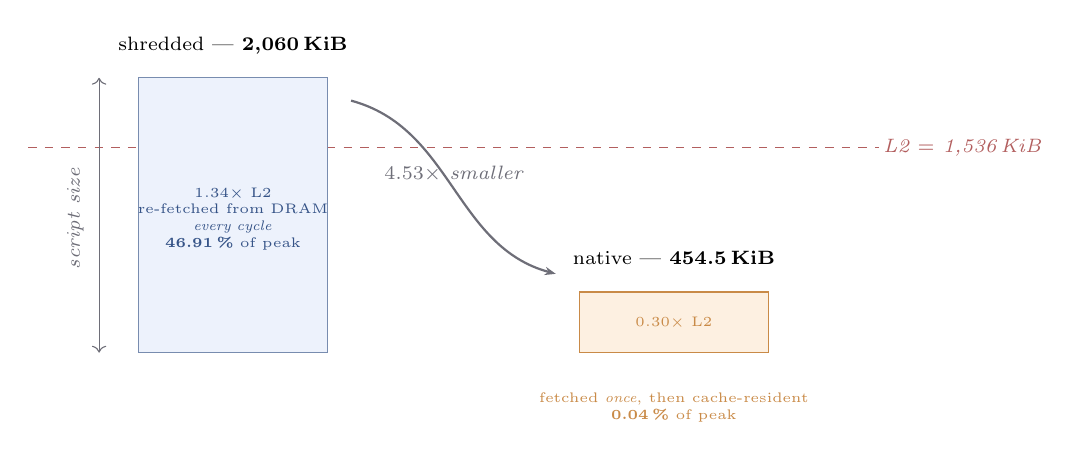
\begin{tikzpicture}[x=1mm,y=1mm]
\draw[draw=rline,thin,dashed] (-4,26) -- (104,26);
\node[lbl,text=rline,right] at (104,26) {L2 $=$ 1,536\,KiB};
\fill[cbox,draw=cline] (10,0) rectangle (34,34.9);
\node[font=\scriptsize,align=center] at (22,39) {shredded --- \textbf{2,060\,KiB}};
\node[font=\tiny,align=center,text=cline!150] at (22,17)
  {$1.34\times$ L2\\re-fetched from DRAM\\\emph{every cycle}\\\textbf{46.91\,\%} of peak};
\fill[mbox,draw=mline] (66,0) rectangle (90,7.7);
\node[font=\scriptsize,align=center] at (78,12) {native --- \textbf{454.5\,KiB}};
\node[font=\tiny,align=center,text=mline] at (78,3.8) {$0.30\times$ L2};
\node[font=\tiny,align=center,text=mline] at (78,-7)
  {fetched \emph{once}, then cache-resident\\\textbf{0.04\,\%} of peak};
\draw[ar,draw=note,thick] (37,32) to[out=-15,in=165] node[lbl,above,pos=0.5]{$4.53\times$ smaller} (63,10);
\draw[<->,draw=note] (5,0) -- (5,34.9);
\node[lbl,rotate=90] at (2,17) {script size};
\end{tikzpicture}
\vspace{5mm}
\caption{Exactly one of the two scripts fits in L2, so the benefit is discontinuous
and the mechanism is residency, not a linear bandwidth saving. The design target is
therefore not ``a smaller script'' but ``a script below 1,536\,KiB''.}
\label{fig:cliff}
\end{figure}

\M{} Measured with \code{cudaGetDeviceProperties} rather than taken from a
specification sheet. Two arithmetic checks confirm the reading:

\begin{itemize}
\item \emph{The baseline's DRAM traffic is essentially all script.} Peak bandwidth is
131.7\,GB/s, so Nsight's $46.91\,\%$ is 61.8\,GB/s; script re-reads alone account for
$2{,}109{,}440\,\mathrm{B} \times 200 / 7.51\,\mathrm{ms} = 56.2$\,GB/s --- $91\,\%$ of
everything measured. The instruction script is not a contributor to the bottleneck;
it \emph{is} the bottleneck.
\item \emph{The native script is fetched approximately once, not two hundred times.}
At $0.04\,\%$ of peak over 15.06\,ms the total DRAM traffic is $\approx 0.8$\,MB,
against a script of 0.465\,MB. Re-reading it every cycle would move 93\,MB.
\end{itemize}

\subsection{Kernel profile}

Nsight Compute, 200 cycles, \code{num\_blocks}$=40$, \code{macro\_bench} at
$\mathrm{LANES}=16$. \I{} The cooperative launch requires
\code{--replay-mode application}: the default per-pass kernel replay re-executes the
kernel in isolation, which a \code{this\_grid().sync()} cannot survive.

\begin{center}\small
\begin{tabular}{lrrl}
\toprule
Metric & Shredded & Native & Reading\\
\midrule
\code{dram\_\_throughput} (\% peak)        & 46.91 & \textbf{0.04} & bandwidth-bound $\to$ not\\
\code{sm\_\_warps\_active} (\% peak)       & 33.33 & 33.33 & occupancy identical\\
\code{smsp\_\_thread\_inst\_executed}      & 28.91 & 19.78 & of 32; the divergence trade\\
Local ld/st sectors                        & 0 & 0 & no spilling\\
\code{gpu\_\_time\_duration} (200 cycles)  & 7.51\,ms & 15.06\,ms & $+37.75\,\mu$s/cycle\\
\bottomrule
\end{tabular}
\end{center}

The warp-divergence row is the deliberate trade this architecture makes. The
boomerang tree is perfectly uniform, so the baseline keeps 28.91 of 32 lanes busy per
issued instruction; a macro batch activates one lane per macro, dropping the native
path to 19.78. Idle arithmetic lanes are bought in exchange for memory traffic --- and
the DRAM row shows the purchase was made in full.

\subsection{Where the remaining time goes}

The measurements decompose cleanly, and three of the four candidate causes are
eliminated by measurement rather than by argument:

\begin{center}\small
\begin{tabular}{@{}lll@{}}
\toprule
Candidate cause & What we measured & Verdict\\
\midrule
Memory bandwidth      & DRAM $46.91\,\% \to 0.04\,\%$ of peak        & \M{} \textbf{Eliminated} --- traffic fell $1{,}173\times$\\
Register spilling     & local ld/st $=0$; \code{STACK:0 LOCAL:0}     & \M{} \textbf{Eliminated} --- nothing spills\\
Occupancy loss        & \code{sm\_\_warps\_active} $=33.33\,\%$ in \emph{both} & \M{} \textbf{Eliminated} --- residency identical\\
Warp divergence       & $28.91 \to 19.78$ of 32 threads/instruction  & \M{} Real, but a small term of a 15.06\,ms kernel\\
Grid synchronisation  & 1 barrier/cycle $\to$ 2                      & \I{} \textbf{Dominant}\\
\bottomrule
\end{tabular}
\end{center}

\F{} The extra grid barrier is the only structural difference between the two
configurations that any measured quantity distinguishes. Two independent timings size
it: $37.75\,\mu$s/cycle from Nsight over 200 cycles, and $31.1\,\mu$s/cycle from wall
clock over 400 --- different instruments, different run lengths, agreeing to within
$20\,\%$. \textbf{The macro-preserving path is synchronisation-bound: not
memory-bound, not occupancy-bound.} It pays one additional grid-wide barrier per
simulated cycle, which exceeds the bandwidth it saves at every scale measured so far.

\textbf{What this result is not.} It is not a measurement of native macro evaluation
being a poor idea; it is a measurement of \emph{where the crossover is not yet}.
\Pj{} Fitting the shredded points gives $\approx 32\,\mu$s/cycle fixed plus script
bytes at $\approx 165$\,GB/s marginal, which places the crossover near a 7\,MB
shredded script --- beyond 32 lanes, whose script is 3,830\,KiB. That is an
extrapolation from two intervals and is labelled as one.

\section{Limitations and Next Optimisation}\label{sec:next}

\begin{center}\footnotesize
\begin{tabular}{@{}p{0.27\textwidth}p{0.28\textwidth}p{0.36\textwidth}@{}}
\toprule
Limitation & Evidence & Fix direction\\
\midrule
Slower than baseline: $0.61\times$ at 16 lanes & \M{} \S\ref{sec:bench} & remove the second major stage --- below\\
32-lane native point missing & write-out budget rejected the mapping & \I{} budget now charges in-cone macros; re-measurement not performed\\
Crossover scale is a projection & \Pj{} fit over two intervals & measure at 32 and 64 lanes\\
Slang SystemVerilog frontend not exercised & \code{macro\_bench.sv} written Verilog-2001-shaped & run both flows on an SV-flavoured design under Yosys 0.68\\
Warp utilisation 19.78/32 in the macro phase & \M{} \S\ref{sec:bench} & warp-cooperative macro evaluation; secondary to the barrier\\
No comparison against other pools' submissions & --- & not available at time of writing\\
\bottomrule
\end{tabular}
\end{center}

\textbf{The target follows from the equations.} Equation (4) charges $+1$ major stage
exactly where a combinational macro output enters the boolean domain, and
\S\ref{sec:bench} measures that stage at $31$--$38\,\mu$s per cycle. The optimisation
target is therefore not a faster macro phase, a better memory layout, or reduced
divergence --- all three are already past the point of diminishing return --- but the
removal of that stage boundary.

\textbf{Proposal: level-1 overlay.} \Pj{} The barrier exists because the boomerang tree
communicates through \code{shared\_state} while the macro phase writes
\code{shared\_writeouts}. If a macro result were injected into the tree's level-1
input set \emph{within the same partition}, the consumer cone would evaluate in the
same major stage and $\mathrm{avail}(v)$ would equal $\mathrm{eval}(v)$ for
$v \in \mathcal{O}_c$ --- collapsing equation (4). The native configuration would
retain its $0.04\,\%$ DRAM utilisation and its $33.33\,\%$ occupancy while paying one
barrier instead of two. Whether that is sufficient to cross $1.0\times$ is not
determined by any measurement we hold, so we state no speedup figure for it. The
change replaces the mechanism \S\ref{sec:sched} is built on and would require the full
verification ladder to be re-run; it was scoped and deliberately not attempted, because
shipping it unverified would have been worse than shipping a measured result.

\section{Conclusion}

\I{} We implemented macro-preserving synthesis, a heterogeneous DAG schedule, a
64-bit aligned VRAM layout and native GPU evaluation for \code{DSP48E2},
\code{CARRY4} and \code{SRLC32E} across 1,591 lines of new host and device code,
leaving GEM's boomerang reduction tree unmodified.

\V{} The result is correct: four verification rungs pass at 32,800 port$\times$timestamp
comparisons each, the macro models agree with an independent transcription over 14,552
vectors, and the \code{CARRY4} space is covered exhaustively.

\M{} The representation objective is met and exceeded. AIG cells fall $14.8\times$,
the per-cycle instruction script $4.53\times$, and --- because that reduction carries
the script across the L2 capacity --- DRAM throughput falls from $46.91\,\%$ of peak
to $0.04\,\%$.

\M{} End-to-end throughput is $0.61\times$ the shredded baseline at 16 lanes. \F{} The
deficit is one additional grid synchronisation per simulated cycle, worth
$31$--$38\,\mu$s, established by eliminating memory bandwidth, register spilling and
occupancy against measured data and corroborated by two independent timings.
\Pj{} Removing that stage boundary is the single change the measurements identify.

What this submission demonstrates is a correct heterogeneous architecture whose
performance characteristics are understood quantitatively rather than asserted: we
know what we built, we know it is right, we know precisely what it costs, and we know
which line of the scheduling equations to attack next.

\section{Measurement Provenance}\label{sec:prov}

\begin{center}\footnotesize
\begin{multicols}{2}
\begin{tabular}{@{}ll@{}}
\toprule
Figure & Source\\
\midrule
Cell counts        & \code{synth/check\_macros.sh}\\
Partition counts   & \code{cut\_map\_interactive} log\\
Script size        & \code{flatten.rs} log line\\
Throughput         & \code{bench/throughput.sh}\\
Kernel profile     & \code{bench/profile.sh} (Nsight)\\
Ladder results     & \code{bench/verify\_ladder.sh}\\
\bottomrule
\end{tabular}

\begin{tabular}{@{}ll@{}}
\toprule
Figure & Source\\
\midrule
Registers / local memory & \code{cuobjdump -res-usage}\\
SM count, blocks/SM      & \code{bench/occupancy\_probe.cu}\\
L2, bandwidth            & \code{bench/memory\_probe.cu}\\
Word state, descriptors  & \code{cut\_map\_interactive} log\\
Port agreement           & \code{bench/compare\_vcd.py}\\
Macro model vectors      & \code{csrc/tests/verify\_macros.sh}\\
\bottomrule
\end{tabular}
\end{multicols}
\end{center}

\noindent Kernel time is GEM's own instrumented figure and excludes VCD parsing.
Baseline and native are measured with the identical metric on the identical device.

\end{document}
